\documentclass[12pt]{article}

\usepackage{sbc-template}

\usepackage{graphicx,url}

\usepackage[brazil]{babel}   
%\usepackage[latin1]{inputenc}  
\usepackage[utf8]{inputenc}  
% UTF-8 encoding is recommended by ShareLaTex

\usepackage{url}
\usepackage{cite}
\usepackage{hyperref}

     
\sloppy

\title{Uso de Projetos de Código Aberto 
	\\no Ensino de Inteligência Artificial}

\author{Esdras L. Bispo Jr.\inst{1} }

\address{Instituto de Ciências Exatas (ICET), Regional Jataí\\ Universidade Federal de Goiás (UFG)\\
  BR 364, km 195, nº 3800, CEP 75801-615 -- Jataí -- GO -- Brasil
  \email{bispojr@ufg.br}
}

\begin{document} 

\maketitle

\begin{abstract}
  Something...
\end{abstract}
     
\begin{resumo} 
  Algo...
\end{resumo}


\section{Introdução}

A aprendizagem por projetos consiste em propor aos alunos cenários semelhantes aos do mundo real e conduzi-los através da construção de uma solução possível. A aprendizagem por projetos está fortemente associada aos conceitos de aprendizagem pela prática ({\it learning by doing}) \cite{anzai:1979, schank:1999, benssen:2015}, aprendizagem autêntica \cite{herrington:2000, herrington:2006, lombardi:2007} e educação direta \cite{lakey:2010}. Este trabalho tem como o objetivo apresentar como o uso do desenvolvimento de software livre contribui para o ensino de Inteligência Artificial (IA).

O Bispix\footnote{\url{http://www.github.com/freeufg/bispix}} é um software livre que foi criado para a realização de projetos na disciplina de IA. O propósito é de que os alunos desenvolvam extensões do Bispix utilizando o modelo de ciclo de vida de software {\it Fork and Pull} \cite{alasbali:2015, buffardi:2015}. Todo o processo é realizado através do GitHub,  permitindo aos alunos o desenvolvimento a partir de um código pré-existente (algo bastante comum no mundo real).

Será apresentado em mais detalhes a seguir alguns conceitos importantes como a aprendizagem pela prática (Seção \ref{sec:doing}), aprendizagem autêntica (Seção \ref{sec:authentic}) e educação direta (Seção \ref{sec:direct}). Logo após, apresentamos o Bispix (Seção \ref{sec:bispix}), e como ele está estruturado. Por fim, apresentamos algumas perspectivas de como gerar resultados de pesquisas interessantes com esta iniciativa (Seção \ref{sec:perspectivas}).

\section{Aprendizagem pelo Fazer} \label{sec:doing}

aprendizagem pela prática ({\it learning by doing}) \cite{anzai:1979, schank:1999, benssen:2015}

\section{Aprendizagem Autêntica} \label{sec:authentic}
\section{Educação Direta} \label{sec:direct}
\section{Bispix} \label{sec:bispix}
\section{Perspectivas de Pesquisa} \label{sec:perspectivas}

\section{First Page} \label{sec:firstpage}

The first page must display the paper title, the name and address of the
authors, the abstract in English and ``resumo'' in Portuguese (``resumos'' are
required only for papers written in Portuguese). The title must be centered
over the whole page, in 16 point boldface font and with 12 points of space
before itself. Author names must be centered in 12 point font, bold, all of
them disposed in the same line, separated by commas and with 12 points of
space after the title. Addresses must be centered in 12 point font, also with
12 points of space after the authors' names. E-mail addresses should be
written using font Courier New, 10 point nominal size, with 6 points of space
before and 6 points of space after.

The abstract and ``resumo'' (if is the case) must be in 12 point Times font,
indented 0.8cm on both sides. The word \textbf{Abstract} and \textbf{Resumo},
should be written in boldface and must precede the text.

\section{CD-ROMs and Printed Proceedings}

In some conferences, the papers are published on CD-ROM while only the
abstract is published in the printed Proceedings. In this case, authors are
invited to prepare two final versions of the paper. One, complete, to be
published on the CD and the other, containing only the first page, with
abstract and ``resumo'' (for papers in Portuguese).

\section{Sections and Paragraphs}

Section titles must be in boldface, 13pt, flush left. There should be an extra
12 pt of space before each title. Section numbering is optional. The first
paragraph of each section should not be indented, while the first lines of
subsequent paragraphs should be indented by 1.27 cm.

\subsection{Subsections}

The subsection titles must be in boldface, 12pt, flush left.

\section{Figures and Captions}\label{sec:figs}


Figure and table captions should be centered if less than one line
(Figure~\ref{fig:exampleFig1}), otherwise justified and indented by 0.8cm on
both margins, as shown in Figure~\ref{fig:exampleFig2}. The caption font must
be Helvetica, 10 point, boldface, with 6 points of space before and after each
caption.

\begin{figure}[ht]
\centering
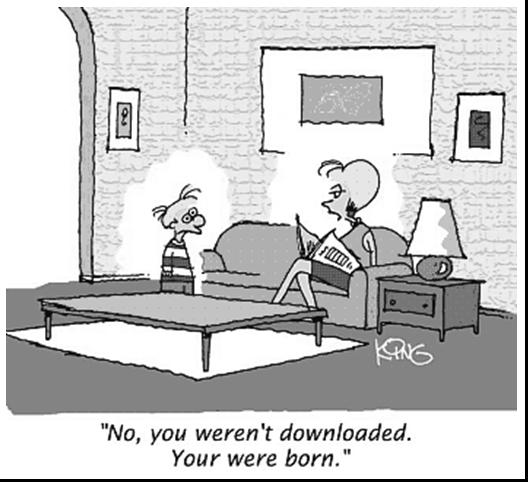
\includegraphics[width=.5\textwidth]{fig1.jpg}
\caption{A typical figure}
\label{fig:exampleFig1}
\end{figure}

\begin{figure}[ht]
\centering
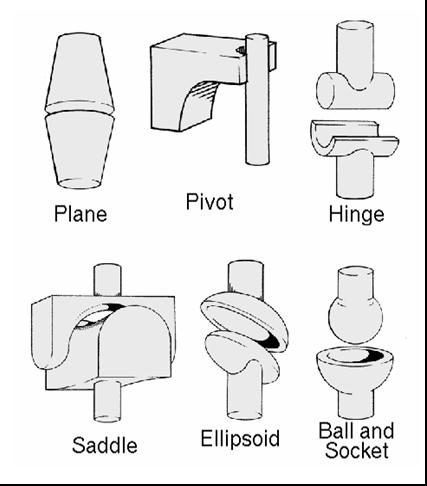
\includegraphics[width=.3\textwidth]{fig2.jpg}
\caption{This figure is an example of a figure caption taking more than one
  line and justified considering margins mentioned in Section~\ref{sec:figs}.}
\label{fig:exampleFig2}
\end{figure}

In tables, try to avoid the use of colored or shaded backgrounds, and avoid
thick, doubled, or unnecessary framing lines. When reporting empirical data,
do not use more decimal digits than warranted by their precision and
reproducibility. Table caption must be placed before the table (see Table 1)
and the font used must also be Helvetica, 10 point, boldface, with 6 points of
space before and after each caption.

\begin{table}[ht]
\centering
\caption{Variables to be considered on the evaluation of interaction
  techniques}
\label{tab:exTable1}
\smallskip
\begin{tabular}{|l|c|c|}
\hline
& Value 1 & Value 2\\[0.5ex]
\hline
&&\\[-2ex]
Case 1 & 1.0 $\pm$ 0.1 & 1.75$\times$10$^{-5}$ $\pm$ 5$\times$10$^{-7}$\\[0.5ex]
\hline
&&\\[-2ex]
Case 2 & 0.003(1) & 100.0\\[0.5ex]
\hline
\end{tabular}
\end{table}

\section{Images}

All images and illustrations should be in black-and-white, or gray tones,
excepting for the papers that will be electronically available (on CD-ROMs,
internet, etc.). The image resolution on paper should be about 600 dpi for
black-and-white images, and 150-300 dpi for grayscale images.  Do not include
images with excessive resolution, as they may take hours to print, without any
visible difference in the result. 

\section{References}

Bibliographic references must be unambiguous and uniform.  We recommend giving
the author names references in brackets, e.g. \cite{knuth:84},
\cite{boulic:91}, and \cite{smith:99}.

The references must be listed using 12 point font size, with 6 points of space
before each reference. The first line of each reference should not be
indented, while the subsequent should be indented by 0.5 cm.

\bibliographystyle{sbc}
\bibliography{bibliografia}

\end{document}
